\TODO[]{Finish Results }
\TODOMaybe{Flesh out more sub-sections}

\draftText{%
  Parse initial study. \\
  Get a feeling for the personas -> observe workflows. \\

  < Manager / Lead >
  \begin{itemize}
    \item{Better overviews}
    \item{Task creation + dispatch}
    \item{Easier input, fewer fields}
    \item{Kanban board for users}
  \end{itemize}

  < Artist >
  \begin{itemize}
    \item{Automation of communication back to manager/lead}
    \item{More collaborative information, "anyone else also working on this?"}
    \item{Auto-completion of information}
    \item{More rigid and centralized info-repository (ex. permanent chat log on
      discussion of specific ticket.)}
    \item{Force information that obscures the process if missing, ex, why is
        this blocked?}
    \item{Easier handling of media uploads, screenshots etc.}
  \end{itemize}

  < Animator >
  \begin{itemize}
    \item{Automatic cascading of skipped tasks -> skip child-tasks}
    \item{Filter or compress similar information}
    \item{Information in flux}
  \end{itemize}

  < System-Architect / Maintainer / Coordinator >
  \begin{itemize}
    \item{Better integration with current tooling}
    \item{Better formatted gantt-chart}
    \item{Batch creation of tasks}
  \end{itemize}
}
\subsection{Initial survey}

  This section presents and analyses the results of the initial survey used in
  order to try to figure out if there are any major grouping that can be turned
  into personas, and what the users think about their initial situation in
  regards to tooling and work-flow.

  \begin{minipage}[b]{0.44\textwidth}
    \begin{figure}[H]
      \centering
        \includegraphics[width=\textwidth]{figures/plots/fig_test.pdf}
        \caption{Hello line subfigure!}
      \end{figure}
  \end{minipage}
  \begin{minipage}[b]{0.49\textwidth}
    \begin{figure}[H]
      \includegraphics[width=\textwidth]{figures/plots/fig_bar_test.pdf}
      \caption{Hello bar subfigure!}
    \end{figure}
  \end{minipage}

%  \begin{wrapfigure}{R}{0.475\textwidth}
%    \centering
%    \includegraphics[width=0.47\textwidth]{figures/plots/fig_pie_test.pdf}
%    \caption{Hello pie subfigure!}
%  \end{wrapfigure}

  \vspace{0.2cm}
  The survey consists of four questions, that are either [M]andatory or
  [O]ptional, and a comment box where comments about the survey or other
  thoughts can be left. Distribution is done by creating a unique link for each
  survey and emailing it to the participants. In total, 25 survey-links were
  sent to members on the team-email list, which resulted in a total of 16
  submitted answerers. See Figure \ref{fig:ref_fig_survey_initial} on page
  \pageref{fig:ref_fig_survey_initial} for a screenshot of
  the survey as viewed in a web-browser.\\

  Q1: [M] \textbf{Role:} \\
  Presented as a text-input field with the suggestion: \textit{programmer,
    animator, etc.} beneath it. \\

  Q2: [O] \textbf{%
    Write a short description, in your own words, of up to three
    work-flow tasks that you often perform in Shotgun:
  } \\
  Question is presented as three text-input fields numbered 1 to 3.\\

  Q3: [O] \textbf{%
    Mark all words that reflect your thoughts on working with \\Shotgun.
  } \\
  Question is presented as a grid of 12 checkboxes representing a word each, the
  layout is scrambled based on the participants name. \\

  Q4: [O] \textbf{%
    Describe up to four work-flow related functionalities that would benefit
    your work if they existed.
  } \\
  Question is presented as four text-input fields numbered 1 to 4.\\

  CB: \textbf{%
    Any comments about the survey, additional details or assorted thoughts
    go here.
  }\\


\subsection{Persona creation}
  \begin{figure}[H]
    \centering
    \begin{subfigure}[b]{0.475\textwidth}
      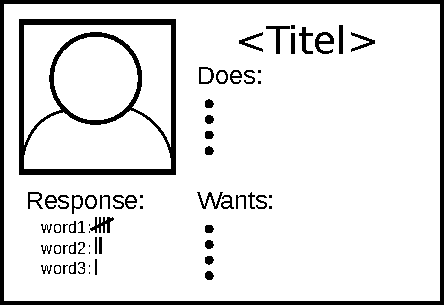
\includegraphics[width=\textwidth]{images/template_persona.pdf}
      \caption{Persona description \#1}
    \end{subfigure}
    \hfill
    \begin{subfigure}[b]{0.475\textwidth}
      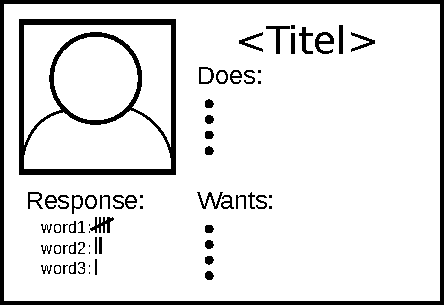
\includegraphics[width=\textwidth]{images/template_persona.pdf}
      \caption{Persona description \#2}
    \end{subfigure}

    \vskip\baselineskip

    \begin{subfigure}[b]{0.475\textwidth}
      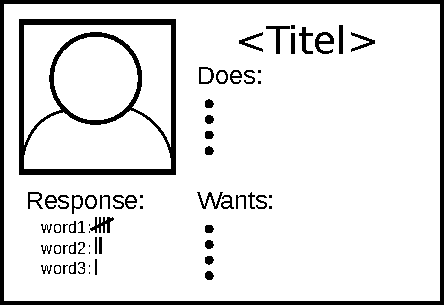
\includegraphics[width=\textwidth]{images/template_persona.pdf}
      \caption{Persona description \#3}
    \end{subfigure}
    \hfill
    \begin{subfigure}[b]{0.475\textwidth}
      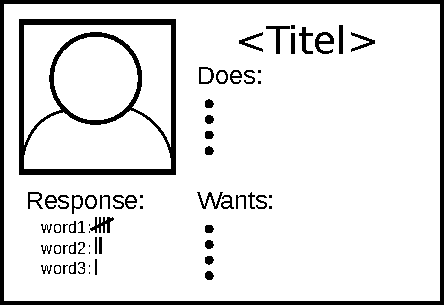
\includegraphics[width=\textwidth]{images/template_persona.pdf}
      \caption{Persona description \#4}
    \end{subfigure}
    \caption{Persona descirptions.}
  \end{figure}
This is the resulting text.
